\subsection*{Motivation}
 %--------------------------------------------------------------------------------------------------
\begin{frame}[t]
    \frametitle{Motivation}
    \framesubtitle{Introductory Examples}
    Consider these situations:
    \begin{figure}
        \centering
        \begin{tikzpicture}[font={\scriptsize}]
            \node (cancer) at (current page.north west) 
                {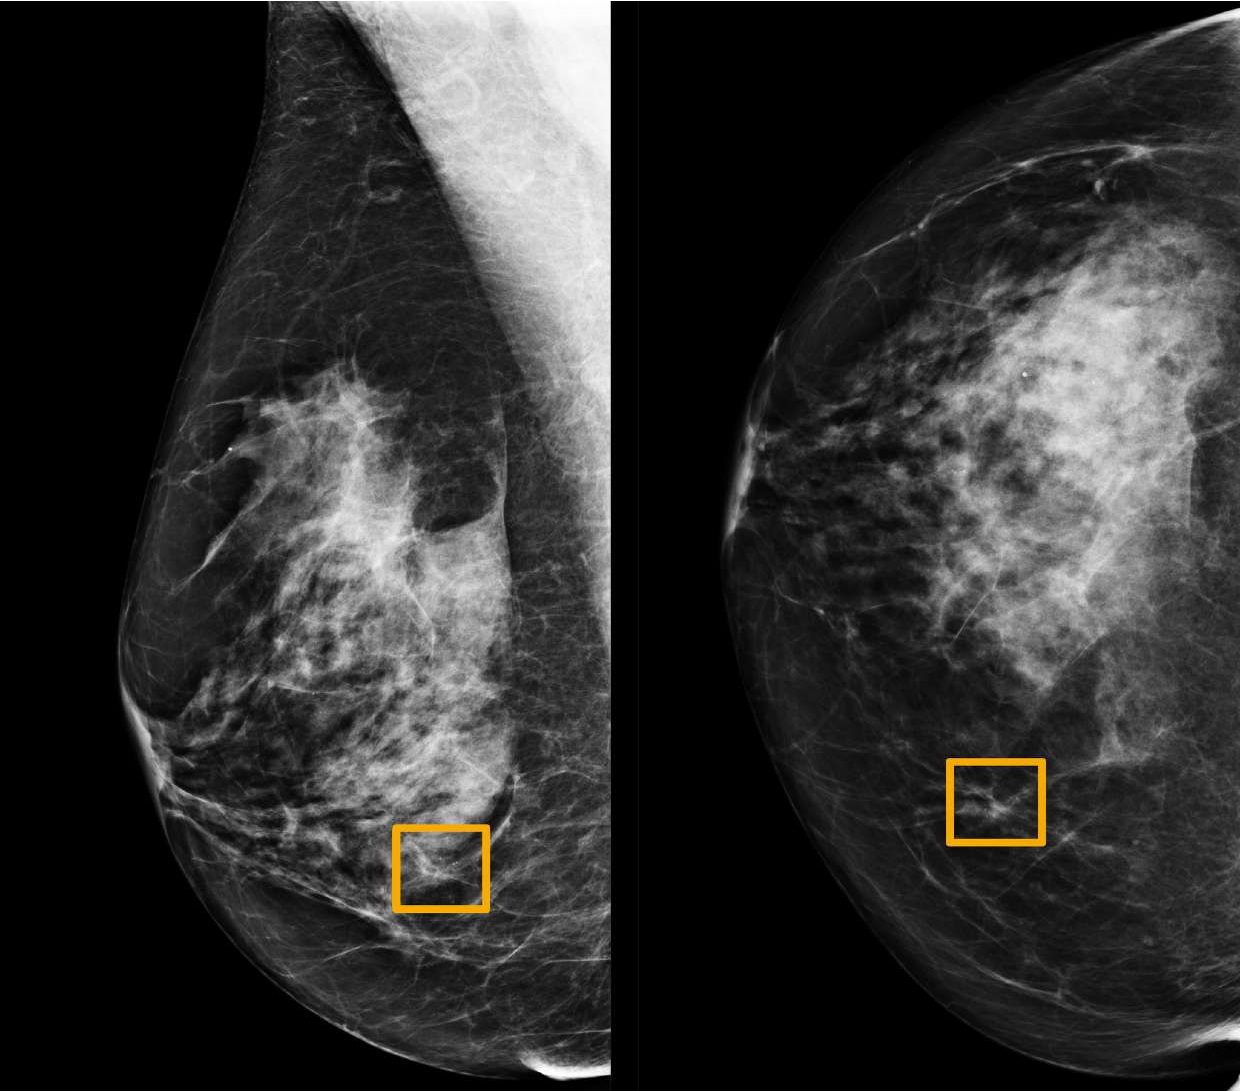
\includegraphics[scale=.2]{fig/intro/motivation/hi_stakes/img/breast_xray.pdf}};
            \pause
            \node (reid) at (cancer.south) {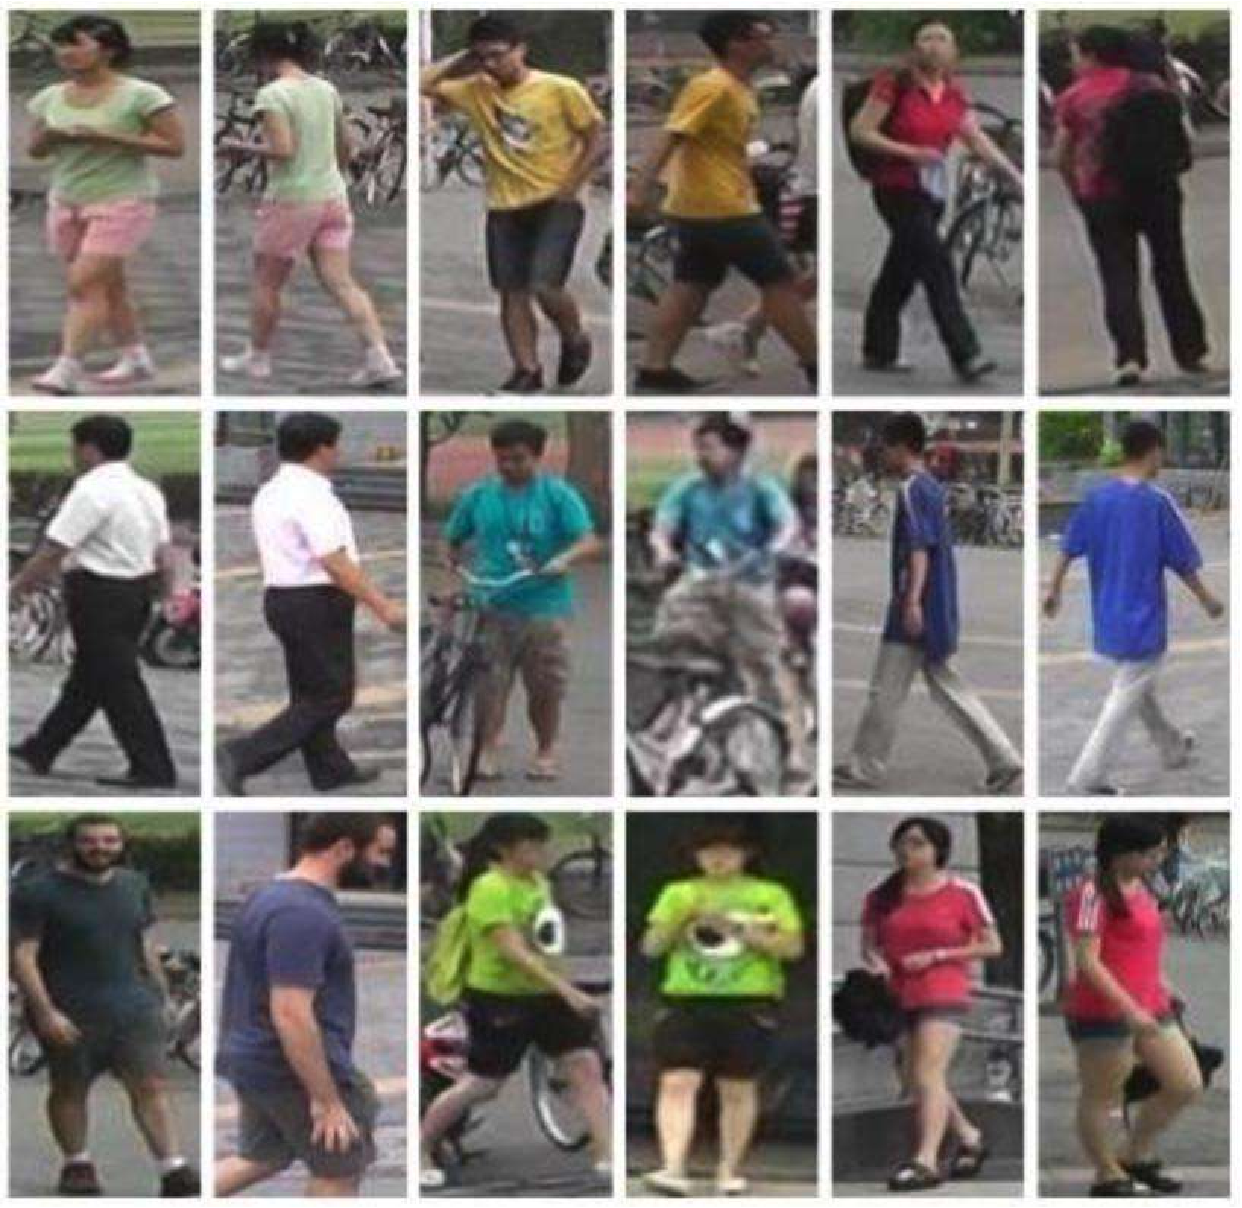
\includegraphics[scale=0.15]
                {fig/intro/motivation/hi_stakes/img/Market-1501.pdf}};
            \pause
            \node (roadkill) at (cancer.east) {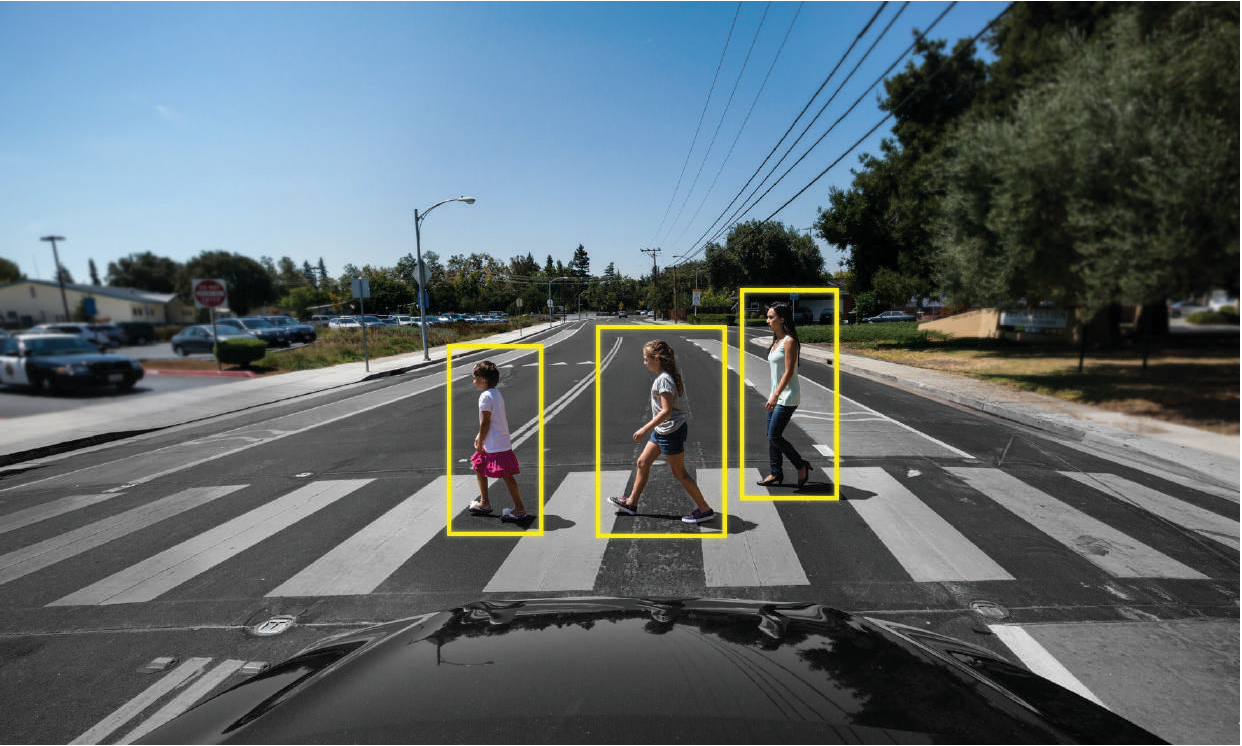
\includegraphics[scale=0.2]
                {fig/intro/motivation/hi_stakes/img/zebra_crossing.pdf}};
            
        \end{tikzpicture}
    \end{figure}
\end{frame}
 %--------------------------------------------------------------------------------------------------
 \begin{frame}[t]
    \frametitle{Motivation}
    \framesubtitle{AI accepted in society?}
    \small
    \begin{columns}[t]
        \column[T]{0.5\textwidth}
        \vspace{30pt}
        \begin{center}
            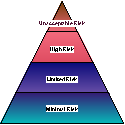
\includegraphics[width=\textwidth]{fig/rel/common/img/risk_pyramid-crop.pdf}\\
            European AI Act for regulation of AI. \cite{madiega2021artificial}    
        \end{center}
        
        \column[T]{0.5\textwidth}
            \begin{itemize}
                \item How do we \textbf{know how} a system works?
                \item How do we \textbf{know how} safe a system is?
                \item If a system fails, \textbf{who} is accountable?
            \end{itemize}
            \pause
            We must \textbf{explain} the behaviour of these models and \textbf{interpret} their predictions.
        \end{columns}
 \end{frame}

 %% Deep Learning